% $Header$

\documentclass{beamer}

% This file is a solution template for:

% - Giving a talk on some subject.
% - The talk is between 15min and 45min long.
% - Style is ornate.



% Copyright 2004 by Till Tantau <tantau@users.sourceforge.net>.
%
% In principle, this file can be redistributed and/or modified under
% the terms of the GNU Public License, version 2.
%
% However, this file is supposed to be a template to be modified
% for your own needs. For this reason, if you use this file as a
% template and not specifically distribute it as part of a another
% package/program, I grant the extra permission to freely copy and
% modify this file as you see fit and even to delete this copyright
% notice. 


\mode<presentation>
{
  %\usetheme{Warsaw}
  %\usetheme{Berlin}
  %\usetheme{metropolis}
  \usetheme{PaloAlto}
  %\usetheme{CambridgeUS}
  %\usetheme{Berkeley}
  
  % font themes
  \usefonttheme{serif}
  %\usefonttheme{structurebold}

  % color themes
  %\usecolortheme{albatross}
  %\usecolortheme{beetle}
  %\usecolortheme{crane}
  %\usecolortheme{dove}
  %\usecolortheme{fly}
  %\usecolortheme{monarca}
  %\usecolortheme{seagull}
  %\usecolortheme{beaver}
  % color themes
  % or ...

  %\setbeamercovered{transparent}
  \setbeamercovered{transparent=5}
  % or whatever (possibly just delete it)
}


\usepackage[english]{babel}
% Place figures exactly where you mean to
%https://tex.stackexchange.com/a/8633/64425
\usepackage{float}
% Place figures exactly where you mean to
% or whatever

\usepackage[utf8]{inputenc}
% or whatever

\usepackage[T1]{fontenc}
% Or whatever. Note that the encoding and the font should match. If T1
% does not look nice, try deleting the line with the fontenc.

% math
\usepackage{amsmath}
\usepackage{amssymb}
\usepackage{amsthm}
% math

% tikz
\usepackage{tikz}
% tikz
\usepackage{caption}
\usepackage{hyperref}
\hypersetup{
    colorlinks,
    linkcolor={magenta!50!black},
    citecolor={blue!50!black},
    urlcolor={blue!80!black}
}
% large commented sections
\usepackage{comment}
% large commented sections



\title[Getting Started with Calculus] % (optional, use only with long paper titles)
{Learning Calculus from the Masters}

\subtitle
{How to Build on Elementary Ideas} % (optional)

\author[Augustus De Morgan, Thomas McCormack, KM] % (optional, use only with lots of authors)
{A.~De Morgan\inst{1} \and T.~McCormack\inst{2}}
% - Use the \inst{?} command only if the authors have different
%   affiliation.

\institute[SDUK] % (optional, but mostly needed)
{
  \inst{1}%
  Original Author
  \and
  \inst{2}%
  First Maintainer
  }
% - Use the \inst command only if there are several affiliations.
% - Keep it simple, no one is interested in your street address.

\date[August 2025] % (optional)
{Aug 2025 / Free Learner's School Conversations}

\subject{Fun Conversations at Home School}
% This is only inserted into the PDF information catalog. Can be left
% out. 



% If you have a file called "university-logo-filename.xxx", where xxx
% is a graphic format that can be processed by latex or pdflatex,
% resp., then you can add a logo as follows:

% \pgfdeclareimage[height=0.5cm]{university-logo}{university-logo-filename}
% \logo{\pgfuseimage{university-logo}}



% Delete this, if you do not want the table of contents to pop up at
% the beginning of each subsection:
\AtBeginSubsection[]
{
  \begin{frame}<beamer>{Outline}
    \tableofcontents[currentsection,currentsubsection]
  \end{frame}
}


% If you wish to uncover everything in a step-wise fashion, uncomment
% the following command: 

%\beamerdefaultoverlayspecification{<+->}


\begin{document}

\begin{frame}
  \titlepage
\end{frame}

\begin{frame}{Outline}
  \tableofcontents
  % You might wish to add the option [pausesections]
\end{frame}


% Since this a solution template for a generic talk, very little can
% be said about how it should be structured. However, the talk length
% of between 15min and 45min and the theme suggest that you stick to
% the following rules:  

% - Exactly two or three sections (other than the summary).
% - At *most* three subsections per section.
% - Talk about 30s to 2min per frame. So there should be between about
%   15 and 30 frames, all told.

% [Kedar] I am keeping this structure, but abusing it to serve my purpose.
% [Kedar] I expect this `presentation' to have many hundred slides, if I end up doing it right.
% [Kedar] There are three sections per presentation, no subsections, but each section may have many, many slides. Let's see. I am just getting started with LaTeX and Beamer.
% [Kedar] I may roughly make a chapter in his book a section in this presentation.
\section{Introduction}
\begin{frame}
\frametitle{Introducing Next Section}
\framesubtitle{In Our Calculus Journey}
\label{slide:intro}
\begin{itemize}
\pause
\item We Continue to Learn from The Masters.
\pause
\item We Started Thinking about Changing Magnitudes And Their Ratios.
\pause
\item You May Wish to Review What We Learned Before.
\end{itemize}
\end{frame}

\section{On The Ratio of Magnitudes \textit{Vanishing} Together}

\begin{frame}
\frametitle{Ratio of Constantly Diminishing Magnitudes}
\framesubtitle{Does It Also Diminish?}
\label{slide:dimmag}
\begin{example}{Two \textit{Diminishing} Magnitudes}
\label{ex:dimlengths}
\begin{itemize}
\pause
\item Consider Two Points A, B on A Curve Below.
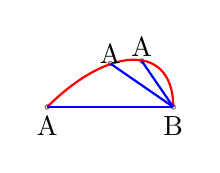
\begin{tikzpicture}[scale=0.8]
\draw [gray] 
  (0,0) circle [radius=1pt] 
  (1,0.69) circle [radius=1pt] 
  (1.5,0.73) circle [radius=1pt] 
  (2,0) circle [radius=1pt];
\draw[thick,red] (0,0) .. controls (1,1) and (2,1) .. (2,0);
\draw (0,0) node[anchor=north] {A};
\draw (1,1.15) node[anchor=north] {A};
\draw (1.5,1.25) node[anchor=north] {A};
\draw (2,0) node[anchor=north] {B};
\draw[thick,blue] (0,0) -- (2,0);
\draw[thick,blue] (1,0.69) -- (2,0);
\draw[thick,blue] (1.5,0.73) -- (2,0);
\end{tikzpicture}
\pause
\item A Approaches B Along The Curve.
\pause
\item Consider Two Lengths: Chord AB, $\overline{AB}$, and Arc AB, $\widehat{AB}$.
\pause
\item As A Approaches B Along The Curve \dots
\begin{itemize}
\pause
\item Isn't It Clear That \alert{Both Magnitudes} $\overline{AB}$, $\widehat{AB}$ \alert{\textbf{Diminish}}?
\pause
\item What Happens to \alert{The Ratio $\frac{\overline{AB}}{\widehat{AB}}$}? Does It \alert{Decrease, Increase, or Remain Constant}?
\end{itemize}
\end{itemize}
\end{example}
\end{frame}

\begin{frame}
\frametitle{Ratio of Constantly Diminishing Magnitudes}
\framesubtitle{Does It Also Diminish?}
\label{slide:dimmag2}
\begin{itemize}
\pause
\item What Happens to The Ratio, \alert{$\frac{A}{B}$}, as $A$ and $B$ Diminish \alert{Is Not Obvious in That Example [\ref{ex:dimlengths}]}, Right?
\pause
\item Although The {Magnitudes Diminish}, The \alert{Ratio Could Remain Constant, Increase, Or Decrease}.
\pause
\item How Could We Ascertain?
\pause
\item Right, We Analyze!
\begin{itemize}
\pause
\item Let's Start with Concrete Cases.
\pause
\item We Consider Discrete Values of The Two Magnitudes as \textit{Corresponding Values of Two Sequences\footnote{Is That A New Word? Well, It Simply Means Values Written One after Another.}}.
\pause
\item Observe How The Values of The Two Magnitudes Change \dots
\pause
\item Remember, The Values \textit{of Both Magnitudes} Are Diminishing.
\item For Simplicity, We May Sometimes Start Both Magnitudes at 1 (Although This Isn't Necessary).
\end{itemize}
\end{itemize}
\end{frame}

\begin{frame}
\frametitle{How The Two Magnitudes Diminish}
\framesubtitle{Do They Diminish Haphazardly?}
\label{slide:mannerofchange}
\begin{itemize}
\pause
\item We Are Studying The Ratio of Diminishing Magnitudes.
\pause
\item However, The Magnitudes Are \alert{Not Diminishing Haphazardly, Whimsically, Or Randomly}.
\pause
\item In The Previous Example, \alert{A Is Constrained to Move along The Predefined Curve as It Approaches B}. 
\begin{itemize}
\item And A Curve Can Be Expressed As A Function Or Formula.
\item \alert{Functions\footnote{You See, Mathematics Borrows This Word From Everyday English And \textit{Redefines} It}}, with Many of Which You Are Familiar, Are Key!  
\end{itemize}
\pause
\item We Use \alert{Sequences of \textit{Corresponding Numbers}} to Aid The Discovery Of Patterns Of Change Or Functions.
\end{itemize}
\end{frame}
\begin{frame}
\frametitle{A Few Words on Sequences of Numbers}
\framesubtitle{Mostly A Matter of Notation \dots}
\label{slide:onseq}
\begin{itemize}
\pause
\item Recall \alert{Arithmetic and Geometric Sequences}?
\pause
\item A Number in A Sequence Is Its \alert{Term}.
\pause
\item The \alert{Order} of Terms of A Sequence Is Crucial.
\pause
\item A Sequence May Have A Finite Number of Terms, e.g.,
\begin{itemize}
\item $1,2,3,4,5$ Represents The Sequence of \alert{Exactly 5 First Counting Numbers}.
\end{itemize}
\pause
\item A Sequence May Have Infinite Terms! Such An \alert{Unending Sequence} Is Shown by The Trailing \dots, e.g.,
\begin{itemize}
\item $1,3,5,7,\dots$ Represents The Sequence of \textit{All} Odd Counting Numbers!
\pause
\item It's Fun to \alert{Guess} The \textit{Pattern of Its Terms}.
\pause
\item A Given Infinite Sequence Should Have Sufficient Number\footnote{The Next Term in $1,2,4,\dots$?} of Terms for Us to Guess The Pattern, If Any!
\end{itemize}
\end{itemize}
\end{frame}


\begin{frame}
\frametitle{Infinite Sequences Are Challenging}
\framesubtitle{And Fun Too!}
\label{slide:infseq}
\begin{itemize}
\pause
\item In Calculus, We Mainly Study Infinite Sequences.
\pause
\item The Idea of Infinity, Denoted by $\infty$, Intrigues, or, Baffles Us.
\pause
\item We Usually Need to Determine The \textit{General Term} of a Sequence as \alert{A Closed-Form Formula\footnote{Is This A New Word? For Now, Think of This as A Function, And You Are Familiar With Functions!} in $n$}.
\begin{itemize}
\item We Denote The General Term of Sequence $S$ by $s_n, n\in\mathbb{N}$.
\end{itemize}
\end{itemize}
\end{frame}

\begin{frame}
\frametitle{Another Thing We Study in Calculus}
\framesubtitle{Among Other Things, of Course!}
\label{slide:rateofchange}
\begin{itemize}
\pause
\item One Magnitude (B) Is Changing. So Is Another (A).
\pause
\item We Want to Find the \alert{Rate} at Which B Changes \alert{with Respect to} A.
\pause
\item We Have Dealt with Such Magnitudes! One Is Displacement (Directed Distance), Another Is Time!
\pause
\item Calculus Provides Us with Means to Study Two Simultaneously Changing Magnitudes.
\pause
\item Therefore, Think of \alert{Rate} of Change of One Thing \alert{wrt} Another!
\end{itemize}
\end{frame}

\begin{frame}
\frametitle{A Slight Digression about \alert{Rate of Change}}
\framesubtitle{Coordinate Plane, Plots, Functions, \dots}
\label{slide:rateofchange2}
\begin{itemize}
\pause \item The Words `Rate' And `Ratio' Are Related.
\pause \item The Coordinate Planes ($XY$, $r\theta$, Etc.) Facilitate The Same: Visualization of Two Simultaneously Changing Magnitudes!
\pause \item You Are Of Course Familiar with `Slope' of A Straight Line
\begin{itemize}
\pause \item The Ratio $\frac{\text{Rise}}{\text{Run}}$.
\pause \item It Is Constant for A Straight Line.
\pause \item Can Be Thought of As \alert{The Rate at Which $Y$ Changes wrt $X$}.
\end{itemize}
\end{itemize}
\end{frame}

\begin{frame}
\frametitle{Back to Sequences}
\label{slide:backtoseq}
{\Large
\alert
{
Back to Sequences of 

Discrete, Simultaneously Diminishing 

Magnitudes \dots
}
}
\end{frame}

\begin{frame}
\frametitle{Our First Sequences of Diminishing Magnitudes}
\framesubtitle{As A And B Diminish, What Happens to $\frac{A}{B}$?}
\label{slide:dimseq}
\begin{itemize}
\pause
\item We Represent Two Diminishing Magnitudes as Sequences $A,B$:
\begin{itemize}
\item $A: 1,\frac{1}{2},\frac{1}{3},\frac{1}{4},\frac{1}{5},\dots$
\item $a_n=\frac{1}{n}$
\item $B: 1,\frac{1}{2},\frac{1}{3},\frac{1}{4},\frac{1}{5},\dots$
\item $b_n=\frac{1}{n}$
\pause
\item Ratio $\frac{A}{B}$: $1,1,1,1,\dots$
\pause
\item The Magnitudes Constantly Diminish, But Their Ratio Remains Constant!
\end{itemize}
\end{itemize}
\end{frame}

\begin{frame}
\frametitle{Another Sequence of Diminishing Magnitudes}
\framesubtitle{As A And B Diminish, What Happens to $\frac{A}{B}$?}
\label{slide:dimseq2}
\begin{itemize}
\pause
\item We Represent Two Diminishing Magnitudes as Sequences $A,B$:
\begin{itemize}
\item $A: 1,\frac{1}{20},\frac{1}{400},\frac{1}{8000},\frac{1}{160000},\dots$
\item $a_n=?$
\item $B: 1,\frac{1}{2},\frac{1}{4},\frac{1}{8},\frac{1}{16},\dots$
\item $b_n=?$
\pause
\item Ratio $\frac{A}{B}$: $1,\frac{1}{10},\frac{1}{100},\frac{1}{1000},\frac{1}{10000},\dots$
\pause
\item The Magnitudes Constantly Diminish, And Their Ratio Also Diminishes!
\pause
\item At Every Step, $A$ Loses Bigger Part of Itself than $B$: $\text{Diminution}_A>\text{Diminution}_B$.
\pause
\item There's No Positive Number, However Small, That Cannot Be Reached by The Ratio!
\pause
\item How Does The Ratio $\frac{B}{A}$ Change?
\end{itemize}
\end{itemize}
\end{frame}

\begin{frame}
\frametitle{One More Sequence of Diminishing Magnitudes}
\framesubtitle{As A And B Diminish, What Happens to $\frac{A}{B}$?}
\label{slide:dimseq3}
\begin{itemize}
\pause
\item We Represent Two Diminishing Magnitudes as Sequences $A,B$:
\begin{itemize}
\item $A: 1,\frac{1}{3},\frac{1}{6},\frac{1}{10},\frac{1}{15},\frac{1}{21},\frac{1}{28},\dots$
\item $a_n=?$
\item $B: 1,\frac{1}{4},\frac{1}{9},\frac{1}{16},\frac{1}{25},\frac{1}{36},\frac{1}{49},\dots$
\item $b_n=?$
\pause
\item Ratio $\frac{A}{B}$: ?
\pause
\item The Magnitudes Constantly Diminish, And Their Ratio ???
\pause
\item What, If Any, Is The \alert {Smallest Value} That The Ratio $\frac{A}{B}$ Will \alert{Never} Achieve? 
\pause
\item How Do You Reason What You See Here?
\begin{itemize}
\item Remember, We Analyze!
\item Might Finding The \alert{General Term} Help?
\item You May Know What We're Getting at \dots
\end{itemize}
\pause
\item How Does The Ratio $\frac{B}{A}$ Change?
\end{itemize}
\end{itemize}
\end{frame}
\section*{Summary}

\begin{frame}{Summary}
\begin{itemize}
\pause
\item Think of Infinite Sequences.
\pause
\item Think of Rate of Change of One Magnitude wrt. Another.
\pause
\item Calculus Began as We Observed Nature, And Tried Reasoning What We Saw. 
\pause
\item We Constantly Experience Change in Nature. Change Is The Only Permanent. 
\pause
\item We Had to Study It Formally.
\end{itemize}
\end{frame}
% ------ copypasta next 5 ------
\begin{frame}
\frametitle{Frame Title}
\framesubtitle{Frame Subtitle}
\label{slide:slidelabel}
\end{frame}
% ------ copypasta prev 5 ------

\begin{comment}
\begin{frame}
\frametitle{There Is No Largest Prime Number}
\framesubtitle{The proof uses \textit{reductio ad absurdum}.}
\begin{theorem}
There is no largest prime number.
\end{theorem}
\begin{proof}
\begin{enumerate}
\item<1-> Suppose $p$ were the largest prime number.
\item<2-> Let $q$ be the product of the first $p$ numbers.
\item<3-> Then $q + 1$ is not divisible by any of them.
\item<1-> But $q + 1$ is greater than $1$, thus divisible by some prime
number not in the first $p$ numbers.\qedhere
\end{enumerate}
\end{proof}
\uncover<4->{The proof used \textit{reductio ad absurdum}.}
\end{frame}

\begin{frame}
\frametitle{What’s Still To Do?}
\begin{columns}[t]
\column{.5\textwidth}
\begin{block}{Answered Questions}
How many primes are there?
\end{block}
\pause
\column{.5\textwidth}
\begin{block}{Open Questions}
Is every even number the sum of two primes?
\cite{Goldbach1742}
\end{block}
\end{columns}
\end{frame}

\begin{thebibliography}{10}
\bibitem{Goldbach1742}[Goldbach, 1742]
Christian Goldbach.
\newblock A problem we should try to solve before the ISPN ’43 deadline,
\newblock \emph{Letter to Leonhard Euler}, 1742.
\end{thebibliography}

\end{comment}

%\begin{frame}{Learn from Masters} %{Subtitles are optional.}
%  % - A title should summarize the slide in an understandable fashion
%  %   for anyone how does not follow everything on the slide itself.
%
%  \begin{itemize}
%  \item
%    Use \texttt{itemize} a lot.
%  \item
%    Use very short sentences or short phrases.
%  \end{itemize}
%\end{frame}
%
%\begin{frame}{Make Titles Informative.}
%
%  You can create overlays\dots
%  \begin{itemize}
%  \item using the \texttt{pause} command:
%    \begin{itemize}
%    \item
%      First item.
%      \pause
%    \item    
%      Second item.
%    \end{itemize}
%  \item
%    using overlay specifications:
%    \begin{itemize}
%    \item<3->
%      First item.
%    \item<4->
%      Second item.
%    \end{itemize}
%  \item
%    using the general \texttt{uncover} command:
%    \begin{itemize}
%      \uncover<5->{\item
%        First item.}
%      \uncover<6->{\item
%        Second item.}
%    \end{itemize}
%  \end{itemize}
%\end{frame}
%
%
%\subsection{Second Subsection}
%
%\begin{frame}{Make Titles Informative.}
%\end{frame}
%
%\begin{frame}{Make Titles Informative.}
%\end{frame}
%
%
% [Kedar] Only one section in this presentation.
% [Kedar] No subsections, sections have slides.


\begin{comment}

\section*{Summary}

\begin{frame}{Summary}

  % Keep the summary *very short*.
  \begin{itemize}
  \item
    The \alert{first main message} of your talk in one or two lines.
  \item
    The \alert{second main message} of your talk in one or two lines.
  \item
    Perhaps a \alert{third message}, but not more than that.
  \end{itemize}
  
  % The following outlook is optional.
  \vskip0pt plus.5fill
  \begin{itemize}
  \item
    Outlook
    \begin{itemize}
    \item
      Something you haven't solved.
    \item
      Something else you haven't solved.
    \end{itemize}
  \end{itemize}
\end{frame}

\end{comment}

\end{document}


